% !TEX encoding = UTF-8 Unicode
%----------------------------------------
\documentclass[english,12pt,a4paper]{article}
%----------------------------------------
%
%----------------------------------------
% !TEX root = FemM1.tex
%----------------------------------------


%----------------------------------------
\usepackage{amsmath,amssymb,amsthm,latexsym}
%\usepackage{stmaryrd}
%\usepackage{pifont}
\usepackage{mathtools}
%\usepackage{refcheck}
\usepackage{hyperref}
%%----------------------------------------
%\usepackage[utf8]{inputenc}
\usepackage{palatino,eulervm}
%---------------------------------------------------------
\usepackage{url}
\usepackage[english,algoruled,lined]{algorithm2e}
\usepackage{listings}
\usepackage{xcolor}
\usepackage[many]{tcolorbox}
\tcbuselibrary{breakable}
\usepackage{xcolor}
\usepackage{cancel}
\usepackage{mathtools} 
\usepackage{enumitem}

% !TEX root = FemM1.tex
%----------------------------------------


%----------------------------------------

\definecolor{myyellow}{rgb}{0.9, 0.9, 0.01}
\definecolor{myblue}{rgb}{0.004, 0.1, 0.57}
\definecolor{myred}{rgb}{0.58, 0.066, 0.}
\definecolor{mygreen}{rgb}{0.24, 0.55, 0.15}
\definecolor{mygray}{rgb}{0.4, 0.6, 0.6}
\definecolor{myviolet}{rgb}{0.3, 0.1, 0.4}
\definecolor{myorange}{rgb}{0.4654205607476635, 0.33271028037383177, 0.20186915887850468}
\newcommand{\blue}[1]{\textcolor{myblue}{#1}}
\newcommand{\red}[1]{\textcolor{myred}{#1}}
\newcommand{\green}[1]{\textcolor{mygreen}{#1}}
\newcommand{\gray}[1]{\textcolor{mygray}{#1}}
\newcommand{\violet}[1]{\textcolor{myviolet}{#1}}
\definecolor{greenlight}{rgb}{0.95,1,0.95}
\definecolor{bluelight}{rgb}{0.9,0.9,1}
\definecolor{graylighy}{rgb}{0.975,0.975,0.975}
\definecolor{yellowlight}{rgb}{0.999, 0.999, 0.925}
\definecolor{roselight}{rgb}{0.99, 0.9, 0.95}
%
\newenvironment{blueenv}{\color{myblue}}{}
\newenvironment{greenenv}{\color{mygreen}}{}
\newenvironment{grayenv}{\color{mygray}}{}
\newenvironment{yellow}[1][]{\begin{tcolorbox}[breakable,title={#1} , boxrule=2pt, colback=yellowlight]}{\end{tcolorbox}}
\newenvironment{rose}[1][]{\begin{tcolorbox}[breakable,title={#1} , boxrule=2pt, colback=roselight]}{\end{tcolorbox}}



%---------------------------------------------------------
%
\newtheorem{theorem}{Theorem}
\newtheorem{lemma}{Lemma}
\newtheorem{corollary}{Corollary}
\newtheorem{proposition}{Proposition}
\newtheorem{remark}{Remark}
\newtheorem{example}{Example}
%

%----------------------------------------
\newcommand{\dpfrac}[2]{\frac{\partial #1}{\partial #2}} 
\newcommand{\ddpfracdiag}[2]{\frac{\partial^2 #1}{\partial #2^2}} 
\newcommand{\ddpfrac}[3]{\frac{\partial^2 #1}{\partial #2\partial #3}} 
\newcommand{\dddpfrac}[4]{\frac{\partial^3 #1}{\partial #2\partial #3\partial #4}} 
\newcommand{\dn}[1]{\dpfrac{#1}{n}} 
\newcommand{\dpt}[1]{\dpfrac{#1}{t}} 
\newcommand{\dptt}[1]{\frac{\partial^2 #1}{\partial t^2 }}  
\newcommand{\dbeta}[1]{\dpfrac{#1}{\beta}} 

%----------------------------------------
% OPT
%\newcommand{\argmin}{\operatorname{argmin}}
\DeclareMathOperator*{\argmin}{argmin}
\DeclareMathOperator*{\argmax}{argmax}

%---------------------------------------------------------
%
% AFEM
%
\newcommand{\REF}{{\mbox{\textbf{REF}}}}
\newcommand{\MARK}{{\mbox{\textbf{MARK}}}}
\newcommand{\allmeshes}{{\mathbb H}}
\newcommand{\meshcriterion}{\mathcal C}
%
\newcommand{\Csolve}{C_{\rm s}}
\newcommand{\Cmesh}{C_{\rm mesh}}
\newcommand{\Cclose}{C_{\rm cls}}
\newcommand{\Cref}{C_{\rm ref}}
\newcommand{\Cglobrel}{C_{\rm gr}}
\newcommand{\Cloceff}{C_{\rm le}}
\newcommand{\Copt}{C_{\rm opt}}
\newcommand{\Cneighb}{C_{\rm nei}}
\newcommand{\Cmeshopt}{C_{\rm mopt}}
\newcommand{\Cgeom}{C_{\rm g}}
\newcommand{\Cmeshcrit}{C_{\rm mc}}
\newcommand{\Cmon}{C_{\rm mon}}
\newcommand{\Cemon}{C_{\rm em}}
\newcommand{\Ceststab}{C_{\rm es}}
\newcommand{\Cinv}{C_{\rm inv}}
\newcommand{\qmesh}{q_{\rm m}}
\newcommand{\qsolve}{q_{\rm s}}

\newcommand{\chistop}[1]{{\chi_{#1}^{\rm fin}}}
\newcommand{\DeltaStop}[1]{{\widetilde{\Delta}_{#1}}}
\newcommand{\solvecrit}[1]{{\mathcal S_{#1}}}
\newcommand{\qred}{q_{\rm red}}
\newcommand{\Crel}{C_{\rm rel}}
\newcommand{\Cstab}{C_{\rm stab}}
\newcommand{\Ceff}{C_{\rm eff}}

\newcommand{\Cupp}{C_{\rm up}}
\newcommand{\Clow}{C_{\rm low}}
\newcommand{\true}{{\mathtt{true}}}
\newcommand{\false}{{\mathtt{false}}}

%---------------------------------------------------------
%
\newcommand{\Expt}[1]{{\rm E}(#1)}
\newcommand{\Var}[1]{{\rm Var}(#1)}
%
\renewcommand{\Re}{\rm Re} 
\renewcommand{\Im}{\rm Im}
\newcommand{\N}{\mathbb N}
\newcommand{\R}{\mathbb R}
\newcommand{\Z}{\mathbb Z}
\newcommand{\C}{\mathbb C}
%
% 
\newcommand{\Set}[1]{ \left\{#1\right\}}
\newcommand{\SetDef}[2]{\left\{#1\;\middle|\;#2\right\}} 
\newcommand{\Rest}[2]{{#1}_{|_{#2}}}
\newcommand{\transpose}[1]{#1^{\mathsf{T}}} 
\newcommand{\transposeInv}[1]{#1^{\mathsf{-T}}} 
%
\newcommand{\supp}[1]{\operatorname{supp}\left(#1\right)}
\renewcommand{\div}{\operatorname{div}}
\newcommand{\rot}{\operatorname{rot}}
\newcommand{\diag}{\operatorname{diag}}
\newcommand{\norm}[1]{\left\|#1\right\|}
\makeatletter
\newcommand{\opnorm}{\@ifstar\@opnorms\@opnorm}
\newcommand{\@opnorms}[1]{%
  \left|\mkern-1.5mu\left|\mkern-1.5mu\left|
   #1
  \right|\mkern-1.5mu\right|\mkern-1.5mu\right|
}
\newcommand{\@opnorm}[2][]{%
  \mathopen{#1|\mkern-1.5mu#1|\mkern-1.5mu#1|}
  #2
  \mathclose{#1|\mkern-1.5mu#1|\mkern-1.5mu#1|}
}
\makeatother
\newcommand{\abs}[1]{\left\vert{#1}\right\vert}
\newcommand{\tnorm}[1]{\opnorm{#1}}
\newcommand{\eps}{\varepsilon}
\newcommand{\scp}[2]{\langle#1,#2\rangle}
\newcommand{\Pe}{\mathrm {Pe}}
\newcommand{\Sides}{\mathcal S}
\newcommand{\Cells}{\mathcal K}
\newcommand{\Nodes}{\mathcal N}
\newcommand{\NodesInt}{{\mathcal N}^{int}}
\newcommand{\level}{\operatorname{lev}}
\newcommand{\SidesInt}{\mathcal S^{\rm int}}
\newcommand{\SidesBdry}{\mathcal S^{\partial}}
\newcommand{\Kin}{K^{\rm{\footnotesize{in}}}}
\newcommand{\Kex}{K^{\rm{\footnotesize{ex}}}}
\newcommand{\inS}[1]{{#1}^{\rm{\footnotesize{in}}}_{S}}
\newcommand{\exS}[1]{{#1}^{\rm{\footnotesize{ex}}}_{S}}
\newcommand{\inSs}[1]{{#1}^{\rm{\footnotesize{in}}}}
\newcommand{\exSs}[1]{{#1}^{\rm{\footnotesize{ex}}}}
\newcommand{\meanS}[1]{\left\{\{#1\right\}_{S}}
\newcommand{\jumpS}[1]{\left[#1\right]_{S}}
\newcommand{\jump}[1]{\left[#1\right]}
\newcommand{\mean}[1]{\left\{#1\right\}}
\newcommand{\intS}{\int_{\Sides_{h}}}
\newcommand{\intSInt}{\int_{\SidesInt_{h}}}
\newcommand{\intSBound}{\int_{\SidesBound_{h}}}
%\newcommand{\intK}{\int_{\Cells_{h}}}
\newcommand{\REFLOC}{{\rm REF}}
\newcommand{\AFEM}[1]{\textbf{AFEM}($#1$)}

%
\newcommand{\tesfctu}{\delta\! u}
\newcommand{\udir}{u^{\rm D}}
\newcommand{\vdir}{v^{\rm D}}
\newcommand{\wdir}{w^{\rm D}}
\newcommand{\uh}{u_{h}}
\newcommand{\phih}{\phi_{h}}
\newcommand{\uin}{u^{\rm in}}
\newcommand{\uex}{u^{\rm ex}}
\newcommand{\uhin}{u^{\rm in}_{h}}
\newcommand{\uhex}{u^{\rm ex}_{h}}
\newcommand{\ubar}{\overline{u}}
\newcommand{\ustar}{u^{*}}
\newcommand{\sgn}[1]{\operatorname{sgn}(#1)}
%
\newcommand{\In}[1]{#1^{\rm in}}
\newcommand{\Ex}[1]{#1^{\rm ex}}
\newcommand{\InDe}[2]{#1^{{\rm in}_{#2}}}
\newcommand{\ExDe}[2]{#1^{{\rm ex}_{#2}}}

%====================================================

\title{Parameter identification with ODE models}
\author{Roland Becker}
\date{\today}
\usepackage{environ}

\newcommand{\alphaLM}{\alpha_{\rm LM}}


%====================================================
\begin{document}
%====================================================
\maketitle
\setcounter{tocdepth}{2}
\tableofcontents
%
%
%==========================================
\section{Parameter estimation problem}\label{sec:}
%==========================================
%
We consider a smooth $n$-dimsniosnal ODE depending on parameters $p\in \R^{n_p}$
%
\begin{equation}\label{eq:ode}
u_t(t) = f(p,u(t)) + l(p,t),\quad t\in I=]0,T[,\qquad u(0) = u_0(p)
\end{equation}
%
with weak formulation
%
\begin{equation}\label{eq:weak_form}
u\in H^1(I,\R^n):\quad a(p,u)(v,v_0) = b(p)(v,v_0)\quad\forall (v,v_0)\in L^2(I,\R^n)\times\R^n
\end{equation}
%
with
%
\begin{equation}\label{eq:forms}
a(p,u)(v,v_0) := \int_0^T \scp{u_t - f(p,u)}{v} + \scp{u(0)}{v_0},\quad b(p)(v,v_0) = \int_0^T \scp{l(p)}{v} + \scp{u_0(p)}{v_0}.
\end{equation}
%
We consider the least-squares problem
%
\begin{equation}\label{eq:}
J(p,u) = \frac12 \norm{R(u)}^2 + \frac{\alpha}{2}\norm{p-p_0}^2,\quad R(u):= C(u)-C_0
\end{equation}
%
where $C: H^1(I,\R^n) \to \R^{n_C}$ is a bounded linear observation operator.
%
We suppose that (\ref{eq:ode}) admits a unique solution $u(p)$ and introduce the reduced functional
%
\begin{equation}\label{eq:}
\hat J (p) := J(p,u(p)),\quad \hat C (p):= C(u(p)).
\end{equation}
%
We have
%
\begin{equation}\label{eq:}
\scp{\nabla \hat J(p)}{q} = \scp{\hat R(p)}{\hat C'(p)(q)} + \alpha\scp{p-p_0}{q}
\end{equation}
%
where $\delta u\in H^1(I,\R^n)$ solves for all $(v,v_0)\in L^2(I,\R^n)\times\R^n$
%
\begin{equation}\label{eq:weak_form}
a'_u(p,u)(\delta u, v,v_0) = b'_p(p)(q,v,v_0)-a'_p(p,u)(q, v,v_0).
\end{equation}
%

%
%==========================================
\section{FEM discretization}\label{sec:}
%==========================================
%
We let $\delta=(0=t_0<t_1<\cdots < t_N=T)$ be a partition, $I_k:=]t_{k-1},t_k[$, $\delta_k=:t_k-t_{k-1}$, $1\le k\le N$.
Let $U_{\delta}\subset H^1(I,\R^n)$ and $V_{\delta}\subset L^2(I,\R^n)$ be conforming finite element spaces. We denote by $\tilde u\in U_{\delta}$ a linearization point in order to obtain semi-implicit schemes:
%
\begin{equation}\label{eq:}
a_{\delta}(p,u)(v) := \int_0^T \scp{u' - \left( f(p,\tilde u) + f'_u(p,\tilde u)(u-\tilde u)\right)}{v}
\end{equation}
%
%
\begin{equation}\label{eq:}
\Rest{\tilde u}{I_k} := u(t_{k-1})
\end{equation}
%
We have
%
\begin{equation}\label{eq:}
{a_{\delta}}_u'(p,u)(w, v) := \int_0^T \scp{w' - \left( f'_u(p,\tilde u)( w) + f''_{uu}(p,\tilde u)(\tilde w,u-\tilde u)\right)}{v}
\end{equation}
%
%
%==========================================
\section{General parameter estimation problem}\label{sec:}
%==========================================
%
We consider the state equation
%
\begin{equation}\label{eq:gen_stateeq}
u\in U:\: a(p,u)(v) = l(p)(v)\quad \forall v\in V.
\end{equation}
%
We suppose that (\ref{eq:gen_stateeq}) has a unique solution $u = u(p)$. 

We consider the least-squares problem of minimizing with linear continuous $C:U\to Z$
%
\begin{equation}\label{eq:gen_ls}
J(p) = \frac12 \norm{R(p)}^2 + \frac{\alphaLM}{2}\norm{p-\overline{p}}^2,\quad R(p) := C(u(p))-\overline{C}.
\end{equation}
%
Based on conforming discretizations, we let
%
\begin{align*}
U_{\delta}\subset U,\quad V_{\delta}\subset V,\quad \dim U_{\delta} = \dim V_{\delta} = N_{\delta}.
\end{align*}
%
we define the discrete problems
%
\begin{equation}\label{eq:gen_stateeq_delta}
u_{\delta}\in U_{\delta}:\: a(p,u_{\delta})(v) = l(p)(v)\quad \forall v\in V_{\delta}.
\end{equation}
%
Then assuming unique solvability, we let $u_{\delta}=u_{\delta}(p)$. Then we have the discrete least-squares problem of minimizing
%
\begin{equation}\label{eq:gen_ls_delta}
J_{\delta}(p) = \frac12 \norm{R_{\delta}(p)}^2 + \frac{\alphaLM}{2}\norm{p-\overline{p}}^2,\quad R_{\delta}(p) := C(u_{\delta}(p))-\overline{C}.
\end{equation}
%

Let $u' = u'(p)(q)\in U$ solve for all $v\in V$
%
\begin{equation}\label{eq:gen_tang}
a_u'(p,u)(u', v) = l'_p(p)(q,v) - a'_u(p,u)(q,v)
\end{equation}
%
and
%
\begin{equation}\label{eq:gen_dual}
z\in V:\; a'_u(p,u)(w,z) = C(w)\quad \forall w\in U.
\end{equation}
%
as well as $u'_{\delta}\in U_{\delta}$ and $z_{\delta}\in V_{\delta}$ the corresponding Petrov-Galerkin solutions.
%---------------------------------------
\begin{lemma}\label{lemma:gen_errorinJ}
%
\begin{equation}\label{eq:gen_errorinJ}
J(p) - J_{\delta}(p) \le  \norm{C(u(p)-u_{\delta}(p))}\left( \frac12 \norm{C(u(p)-u_{\delta}(p))} + \norm{R_{\delta}(p)}\right)
\end{equation}
%
\begin{equation}\label{eq:gen_errorinGrad}
%
\begin{aligned}
\norm{\nabla J(p) - \nabla J_{\delta}(p)} \le& \norm{C(u(p)-u_{\delta}(p))}\left( \norm{C(u'(p))} + \norm{C(u'(p)-u'_{\delta}(p))}\right)\\
&+ \norm{R_{\delta}(p)}\norm{C(u'(p)-u'_{\delta}(p))}.
\end{aligned}
%
\end{equation}
%
%
\end{lemma}
%
%---------------------------------------
\begin{proof}
%
\begin{align*}
J(p) - J_{\delta}(p) =&  \frac12 \norm{R(p)}^2 - \frac12 \norm{R_{\delta}(p)}^2 = \frac12 \norm{R(p)-R_{\delta}(p)}^2 + \scp{R(p)-R_{\delta}(p)}{R_{\delta}(p)}\\
=& \frac12 \norm{C(u(p)-u_{\delta}(p))}^2 +  \scp{C(u(p)-u_{\delta}(p))}{R_{\delta}(p)}
\end{align*}
%
and
%
\begin{align*}
\scp{\nabla J(p) - \nabla J_{\delta}(p)}{q} =& \scp{R(p)}{C(u'(p)(q))} - \scp{R_{\delta}(p)}{C(u_{\delta}'(p)(q))} \\
=& \scp{C(u(p)-u_{\delta}(p))}{C(u'(p)(q))} + \scp{R_{\delta}(p)}{C(u'(p)(q)-u_{\delta}'(p)(q))}
\end{align*}
%
\end{proof}
%




\cite{Feischl22}

%
%==========================================
\section{Numerical experiments}\label{sec:}
%==========================================
%
%
%-------------------------------------------------------------------------
\subsection{Bock's example}\label{subsec:}
%-------------------------------------------------------------------------
%
\cite{Bock87}
%
\begin{equation}\label{eq:}
\begin{bmatrix}
u'\\ v'
\end{bmatrix}
=
\begin{bmatrix}
v\\ -p u
\end{bmatrix}
,\quad 
\begin{bmatrix}
u(0)\\ v(0)
\end{bmatrix}
=
\begin{bmatrix}
1\\ 0
\end{bmatrix},\quad
C = 
\begin{bmatrix}
u(T)\\ \int_0^T u(t)
\end{bmatrix},\quad
\overline{C} = 
\begin{bmatrix}
0\\ 2/\pi
\end{bmatrix}
\end{equation}
%
with $T=1$. We use an initial guess $p_0=1$. The  solution is $p^*=\pi$.

\begin{figure}[htbp]
\begin{center}
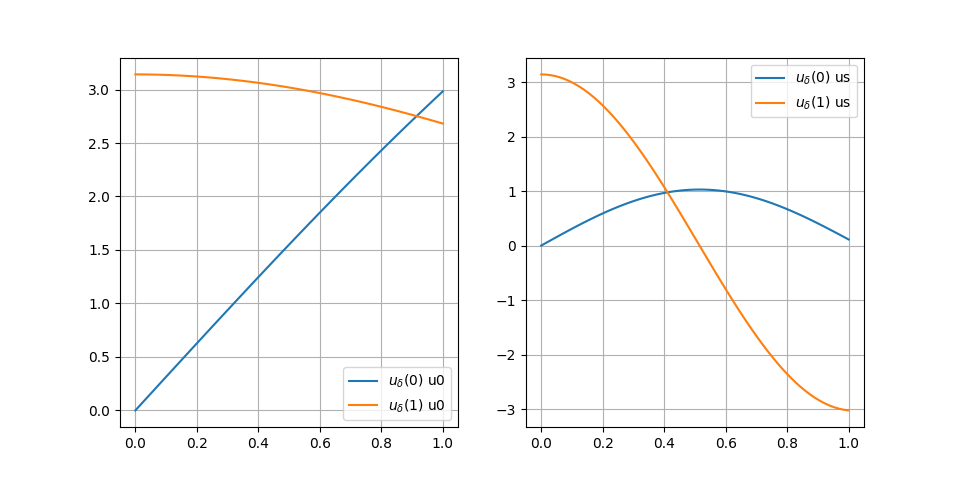
\includegraphics[keepaspectratio = true, width = 0.5\textwidth] {img/bock/u0_us}\hfill
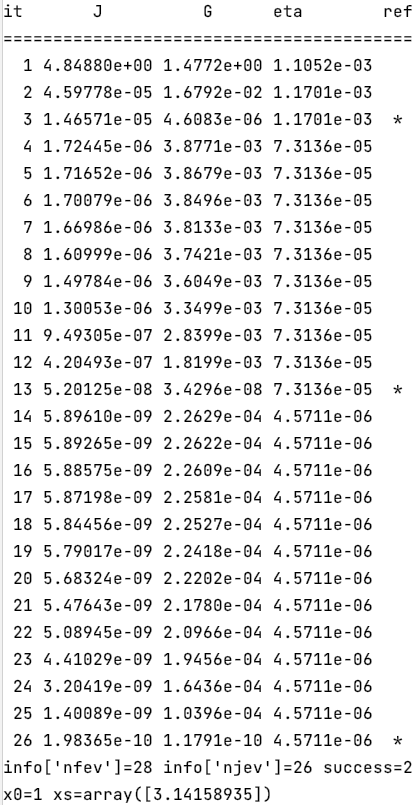
\includegraphics[keepaspectratio = true, width = 0.3\textwidth] {img/bock/info}\\\vspace{5mm}
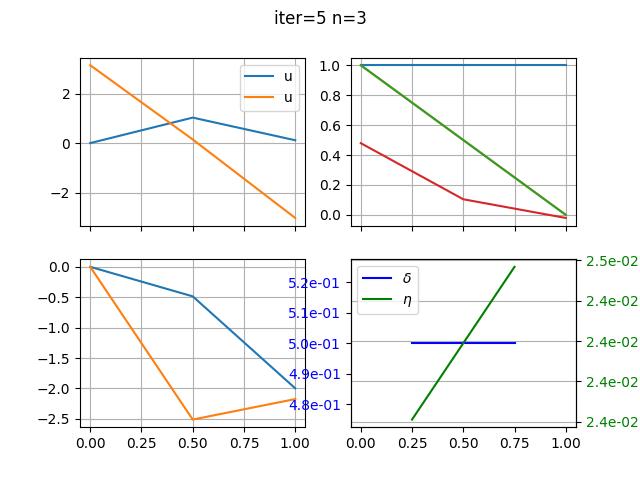
\includegraphics[keepaspectratio = true, width = 0.3\textwidth] {img/bock/iter5}\hfill
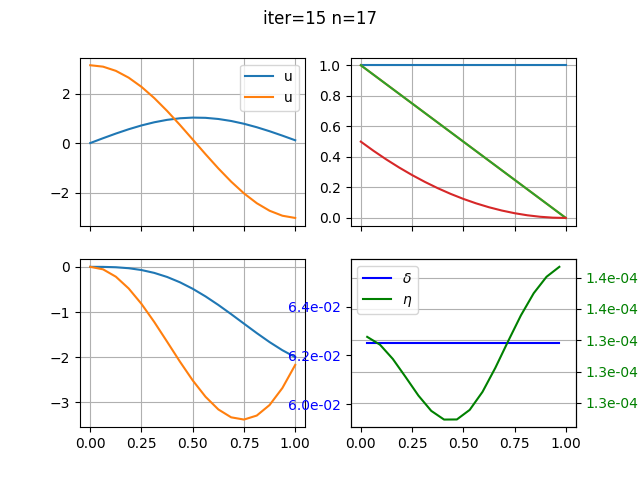
\includegraphics[keepaspectratio = true, width = 0.3\textwidth] {img/bock/iter15}\hfill
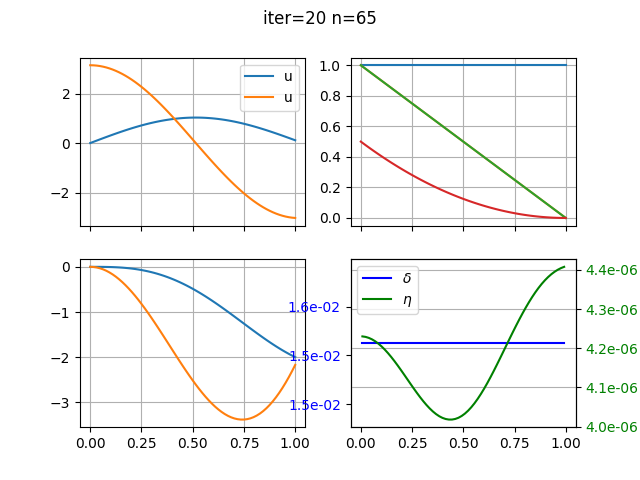
\includegraphics[keepaspectratio = true, width = 0.3\textwidth] {img/bock/iter20}
\caption{Bock's example}
\label{default}
\end{center}
\end{figure}
%
%-------------------------------------------------------------------------
\subsection{Lorenz}\label{subsec:}
%-------------------------------------------------------------------------
\begin{figure}[htbp]
\begin{center}
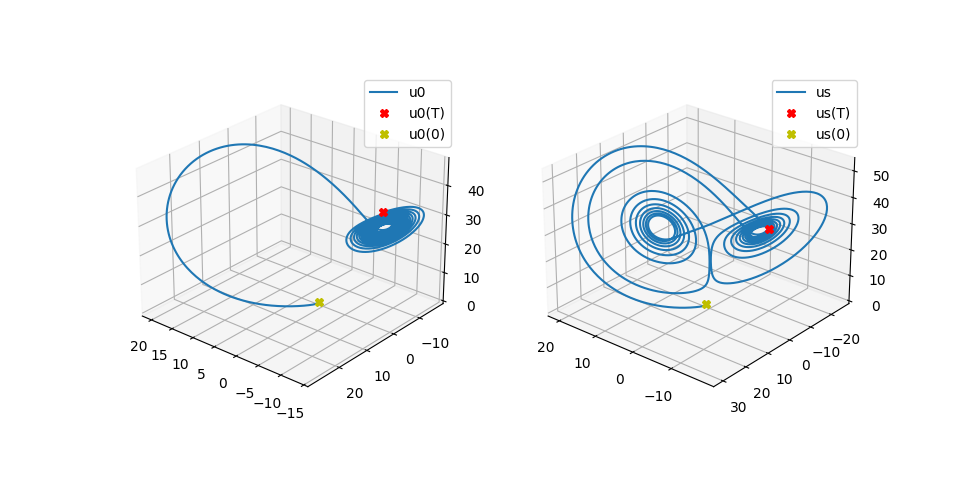
\includegraphics[keepaspectratio = true, width = 0.5\textwidth] {img/lorenz/u0_us}\hfill
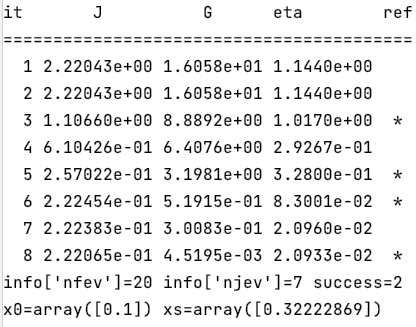
\includegraphics[keepaspectratio = true, width = 0.4\textwidth] {img/osc/info}\\\vspace{5mm}
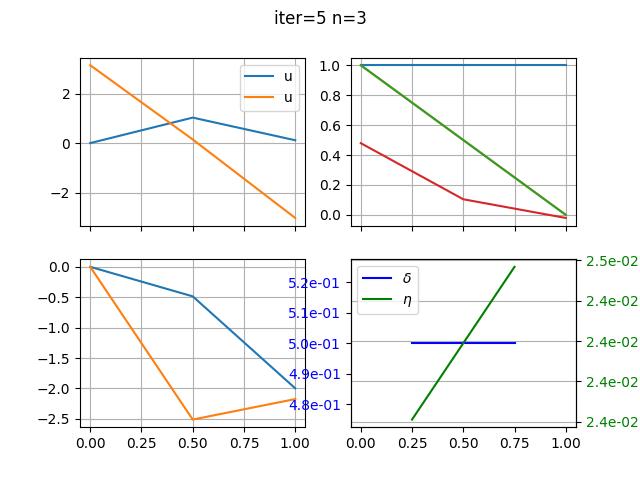
\includegraphics[keepaspectratio = true, width = 0.3\textwidth] {img/bock/iter5}\hfill
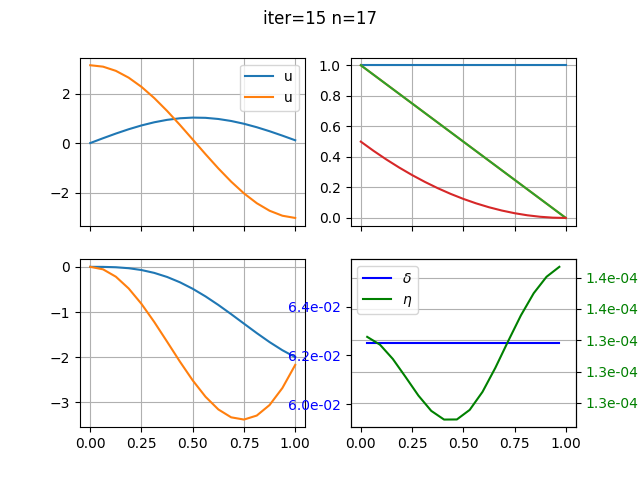
\includegraphics[keepaspectratio = true, width = 0.3\textwidth] {img/bock/iter15}\hfill
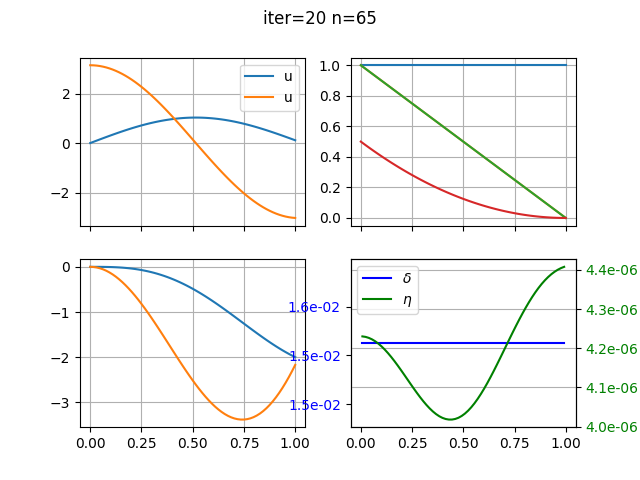
\includegraphics[keepaspectratio = true, width = 0.3\textwidth] {img/bock/iter20}
\caption{Bock's example}
\label{default}
\end{center}
\end{figure}
%

%
%-------------------------------------------------------------------------
\subsection{Oscillator}\label{subsec:}
%-------------------------------------------------------------------------
%
%
\begin{equation}\label{eq:}
\begin{bmatrix}
u'\\ v'
\end{bmatrix}
=
\begin{bmatrix}
v\\ -p u
\end{bmatrix}
,\quad 
\begin{bmatrix}
u(0)\\ v(0)
\end{bmatrix}
=
\begin{bmatrix}
1\\ 0
\end{bmatrix},\quad
C = 
\begin{bmatrix}
u(T)\\ v(T)
\end{bmatrix},\quad
\overline{C} = 
\begin{bmatrix}
1\\ -1
\end{bmatrix}
\end{equation}
%
with $T=12$. We use an initial guess $p_0=0.1$. The closest solution is $p^*\approx0.322$.

\begin{figure}[htbp]
\begin{center}
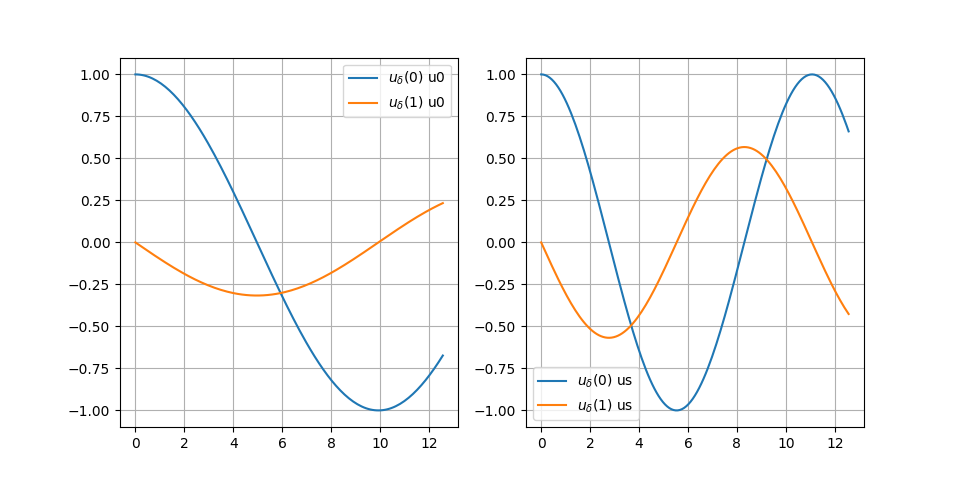
\includegraphics[keepaspectratio = true, width = 0.5\textwidth] {img/osc/u0_us}\hfill
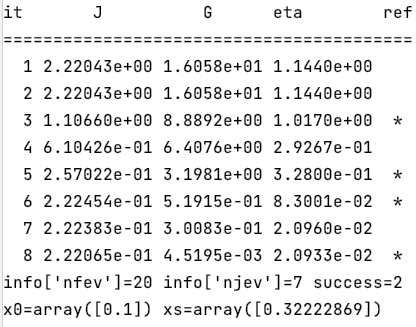
\includegraphics[keepaspectratio = true, width = 0.4\textwidth] {img/osc/info}\\\vspace{5mm}
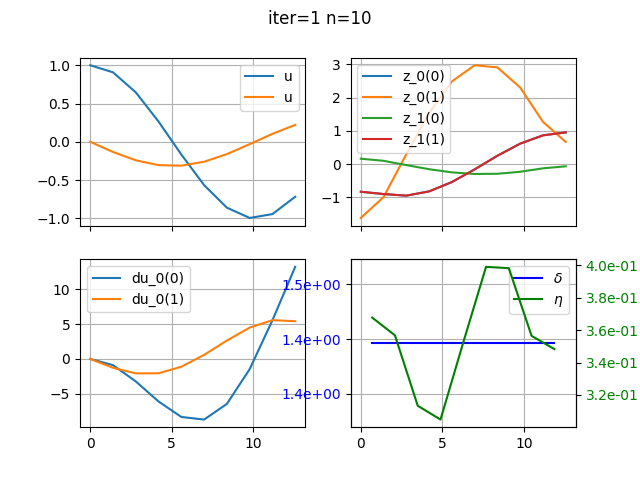
\includegraphics[keepaspectratio = true, width = 0.3\textwidth] {img/osc/iter1}\hfill
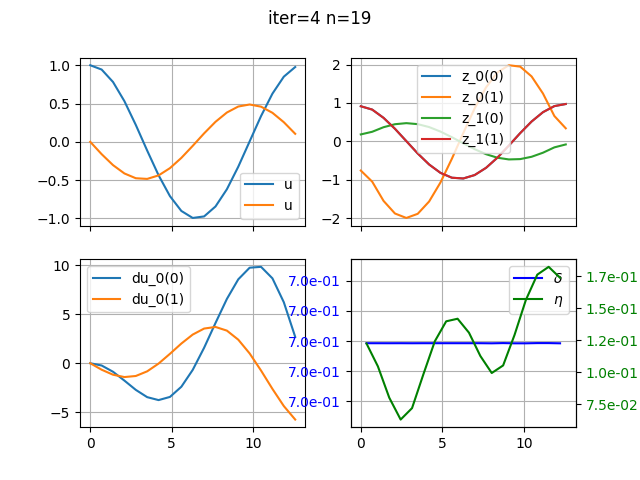
\includegraphics[keepaspectratio = true, width = 0.3\textwidth] {img/osc/iter4}\hfill
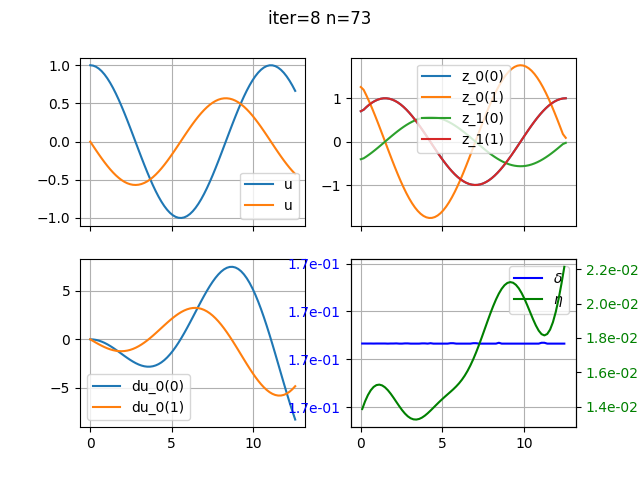
\includegraphics[keepaspectratio = true, width = 0.3\textwidth] {img/osc/iter8}
\caption{default}
\label{default}
\end{center}
\end{figure}



%====================================================


\bibliography{/Users/becker/Latex/Bibliotheque/bibliotheque.bib}
\bibliographystyle{ieeetr}

%====================================================
\end{document}
%===================================================w